\chapter{Results}
\label{sec:results}

The following sections present results from analysis of the verification model, compression performance of the delayed weight update scheme, and performance of the modified hardware design. The \acrshort{hypso}-2 coastline image set is presented in \autoref{app:coastline-images}, consisting of ten images. The images have dimensions $N_z=120$, $N_y=598$ and $N_x=1092$, for a total of $78.36$ million samples, taken at a frame rate of $8$ frames per second. Images from the AVIRIS Yellowstone set have dimensions of $N_z=224$, $N_y=512$, and varying size in the $x$ dimension of $N_x \in \{614, 677, 680\}$, for roughly $77$ million samples.

\section{Verification Model}

\begin{figure}[ht]
	\begin{center}
		\efbox{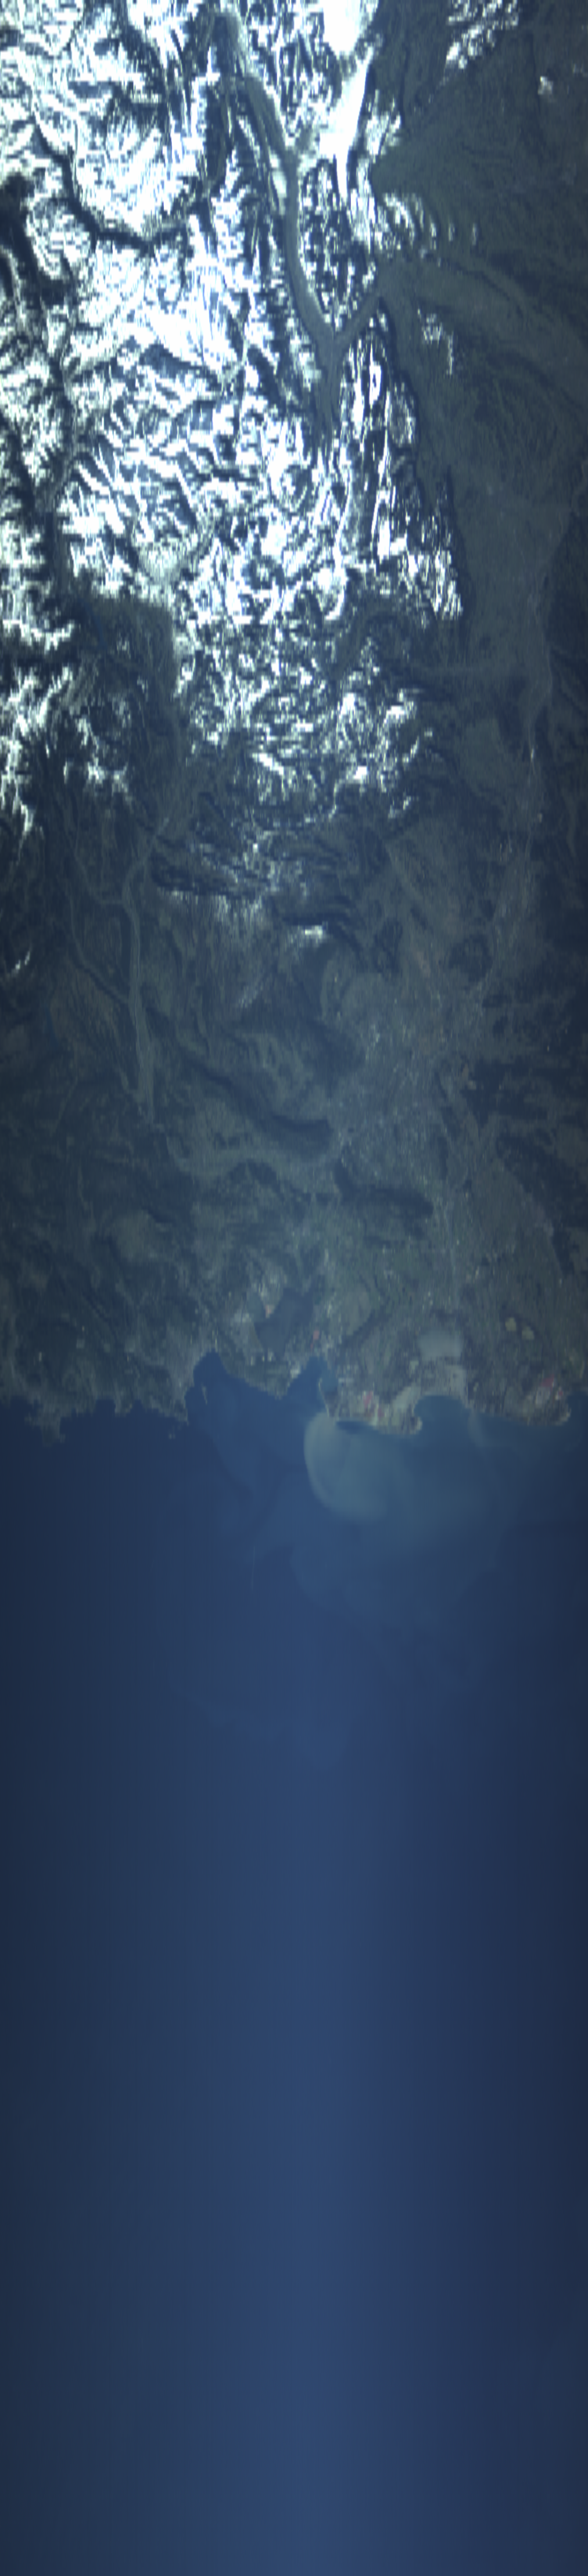
\includegraphics[height=0.28\textheight,valign=t]{figures/hypso2-rgb/hypso_decoded.png}}
		\efbox{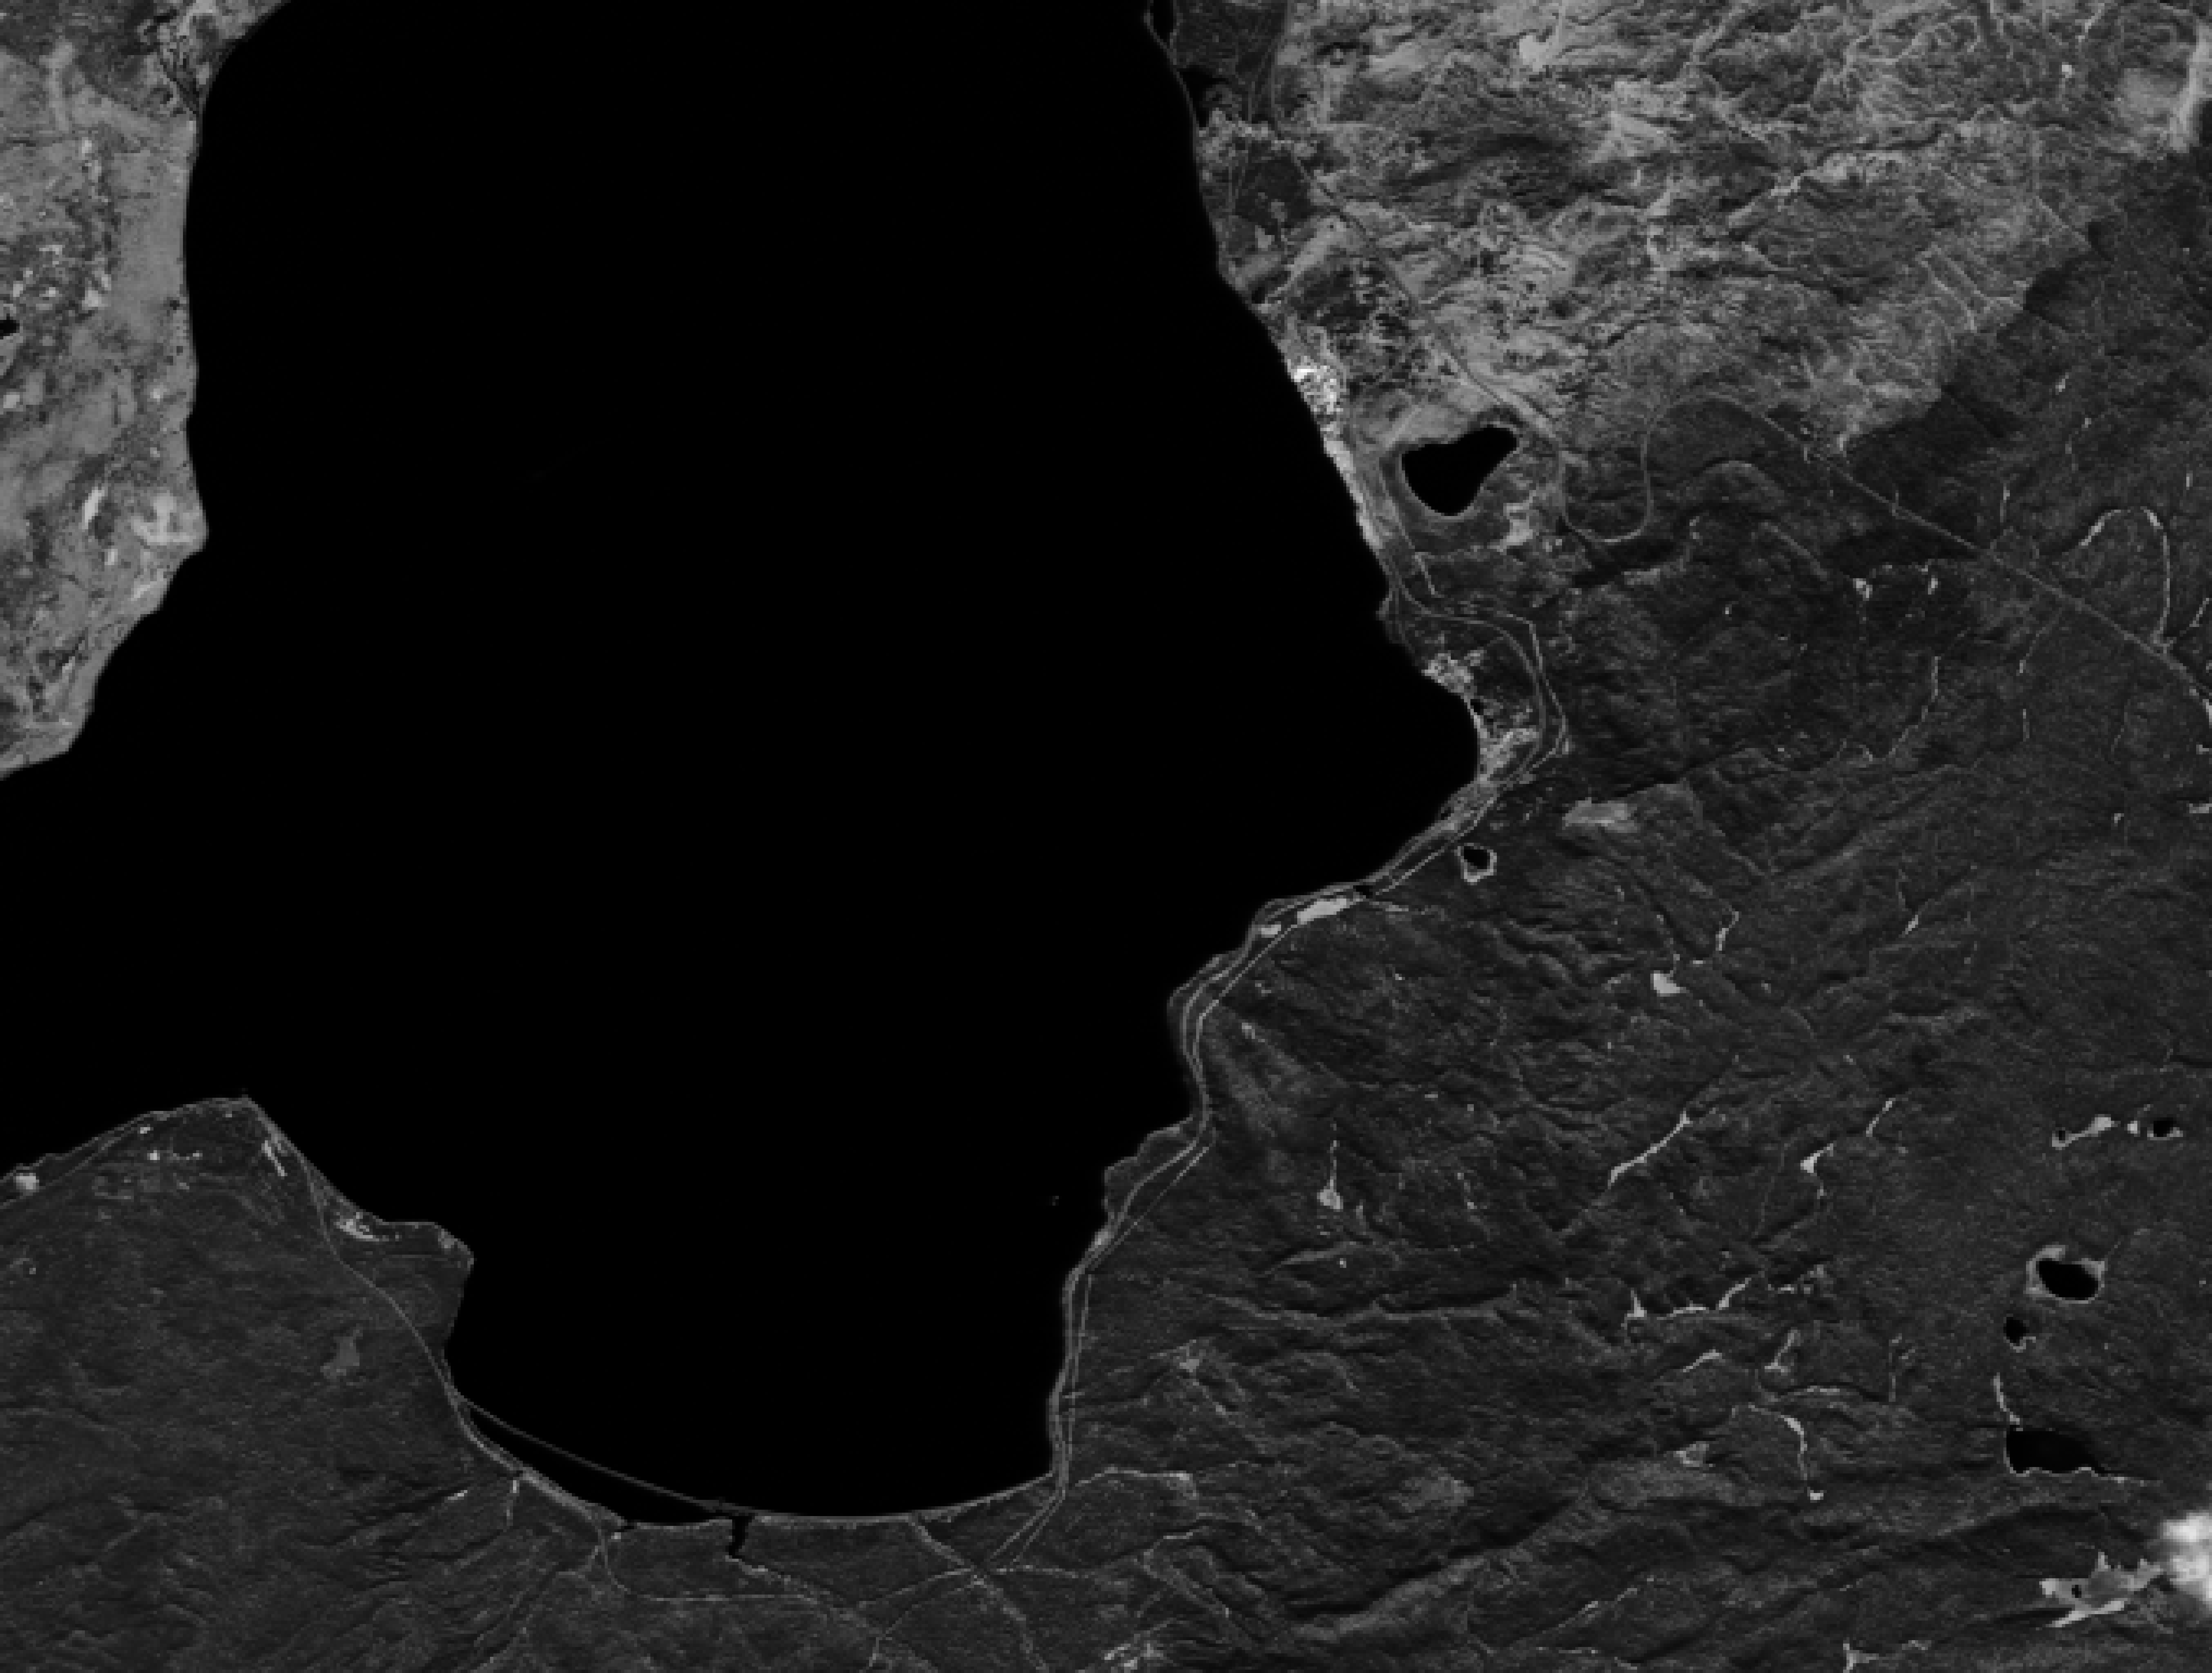
\includegraphics[height=0.28\textheight,valign=t]{results/aviris/aviris_decoded.png}}
		% 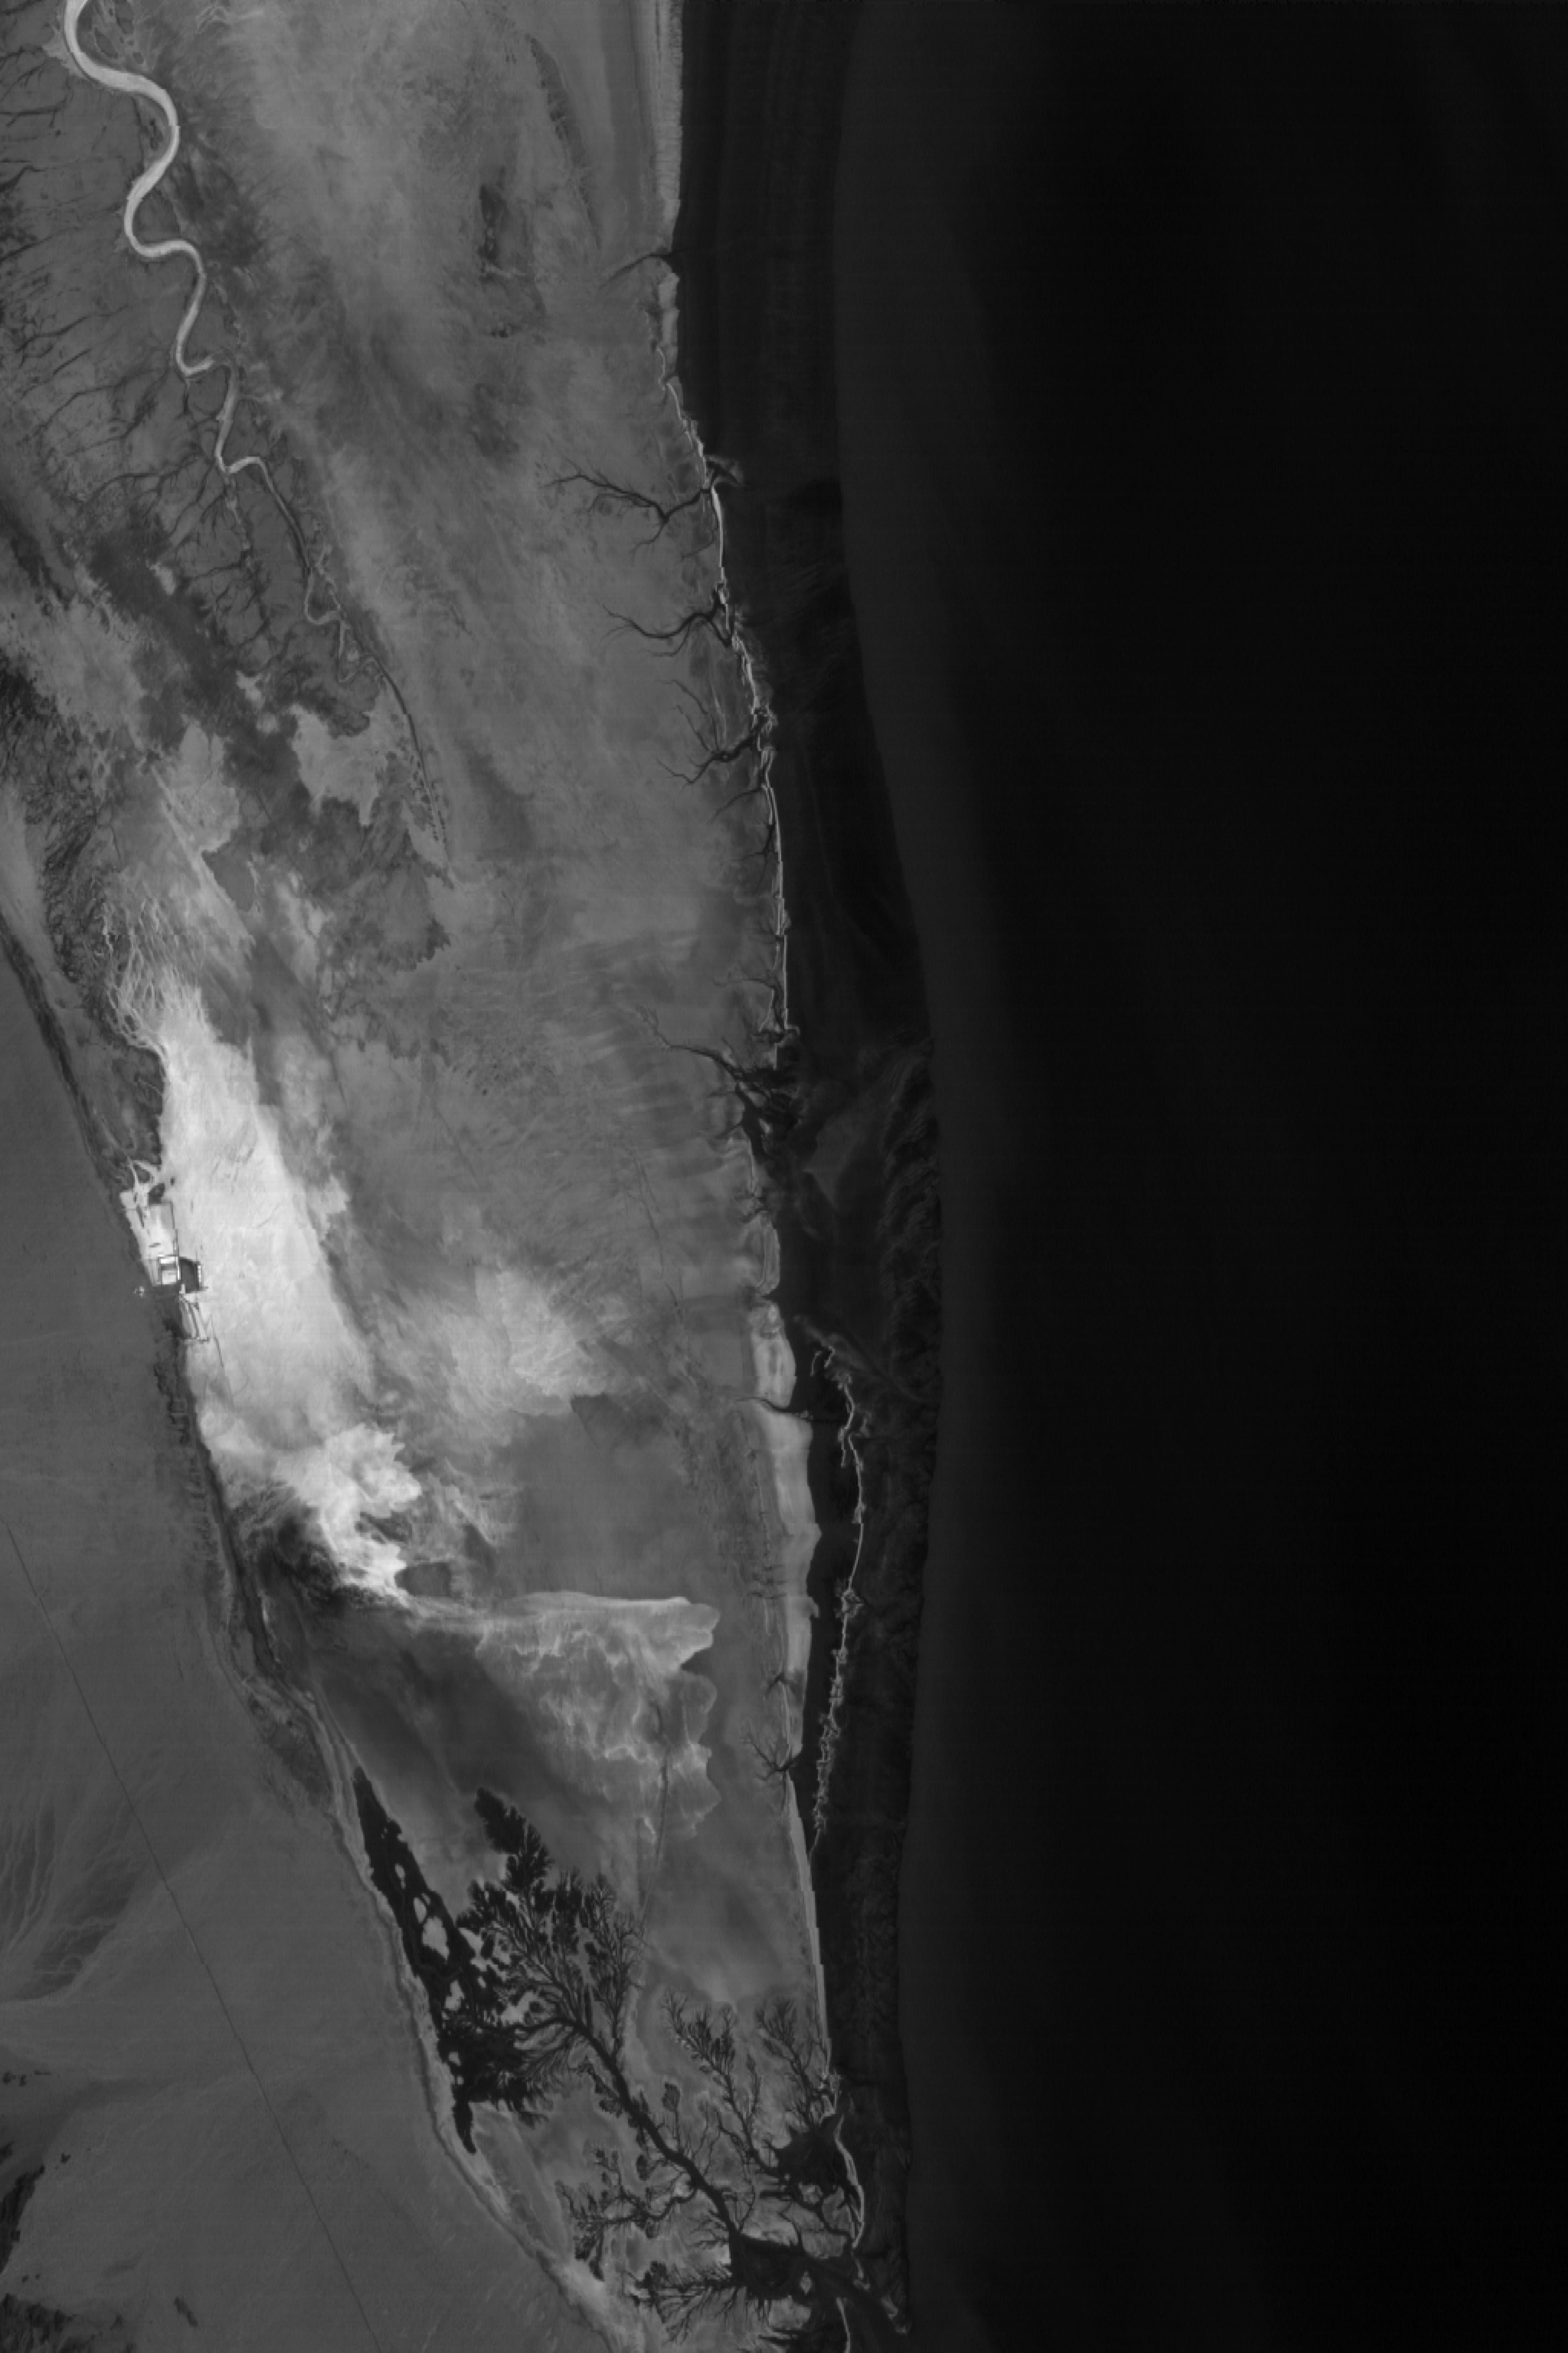
\includegraphics[height=0.28\textheight,valign=t]{results/landsat/landsat_decoded.png}
	\end{center}
	\caption{Two decompressed images from HYPSO-2 and AVIRIS Yellowstone, compressed with delayed weight update scheme with $r_z=16$ and $a_z=4$.}
	\label{fig:decompressed}
\end{figure}

\autoref{fig:decompressed} shows two images from the \acrshort{hypso}-2 coastline and AVIRIS Yellowstone sets that have been compressed and decompressed using the verification model, with delayed weight updates. The images were compressed using $r_z=16$ and $a_z=4$, giving compression ratios of $2.47$ and $4.31$ for HYPSO-2 and AVIRIS images respectively. Visual inspection shows that the verification model can successfully reconstruct the original images, while employing the modified weight update scheme. Additionally, all images from both image sets have been compressed in lossless mode, in which all reconstructed images are identical to the originals.

\begin{figure}[ht]
	\begin{center}
		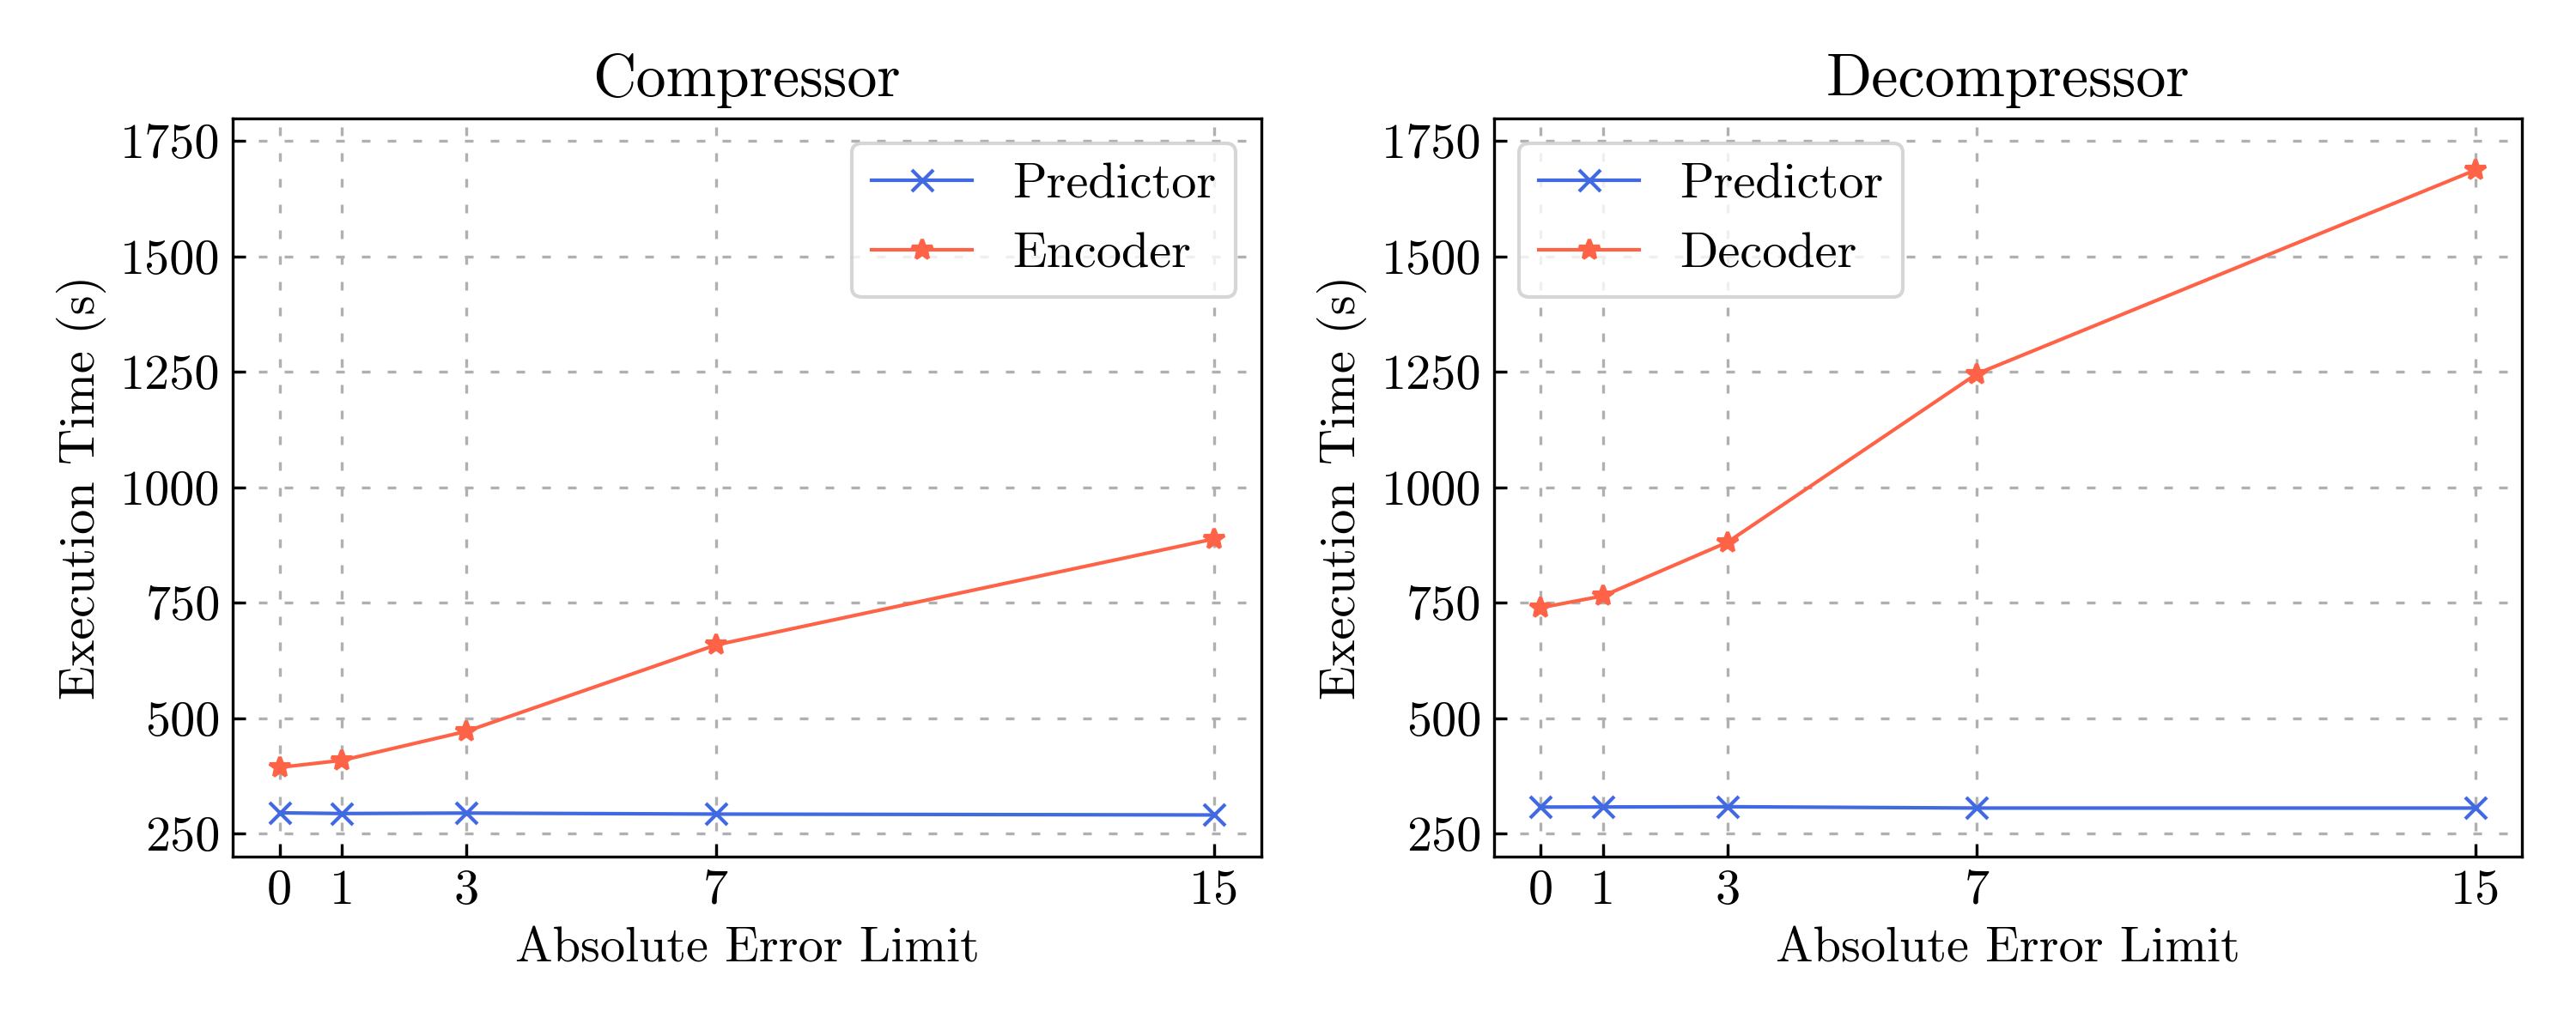
\includegraphics[width=1\textwidth]{figures/execution_time.png}
	\end{center}
	\caption{Execution time for the C++ predictor and hybrid encoder modules during compression and decompression for a set of absolute error limits. Results are averaged over a set of ten \acrshort{hypso}-2 images.}
	\label{fig:execution_time}
\end{figure}

Execution time of the verification model is analysed using the \acrshort{hypso}-2 coastline set, and is averaged across the images for a set of \acrshort{PAE}s. The four main stages of compression/decompression are timed separately: load data, predictor, encoder/decoder, and save data. Tests are run on a computer with an AMD Ryzen 5 3600X CPU and 64 GB of RAM. Tables \ref{tab:coastline-compress} and \ref{tab:coastline-decompress} summarize the execution time results for compression and decompression using the verification model. The same results are visualized in \autoref{fig:execution_time}.

Execution time of the C++ predictor remains more or less constant at $~300$ seconds for both compression and decompression. The hybrid encoder, still written in Python, displays a significant increase in execution time as the absolute error limit is adjusted. This change is most prominent in the decoder stage of the decompressor, with execution times almost double those of the encoder stage of the compressor. The increasing execution times are likely due to the use of \acrshort{V2V} codes as predicted sample entropy decreases for higher absolute error limits.

During compression, execution time for the loading and saving of data to and from the disk is negligible. For the decompressor, saving data takes $~70$ seconds. This is because all image samples must be iterated over and stored to file in the correct sample store order (\acrshort{BIL}, \acrshort{BIP}, \acrshort{BSQ}), as dictated by the header configuration. The compressor can store the compressed bitstream directly to file without modifications.

\autoref{tab:coastline-compress-py} shows execution times for compression using the old predictor module written in Python. The predictor has a runtime of $~2100$ seconds, over seven times slower than that of the C++ predictor. Saving output data also takes significantly longer. This is because the module stores additional, intermediate results, a feature that is made optional in the C++ predictor.

\begin{table}[ht]
	\caption{Performance of compression using verification model with C++ predictor and delayed weight updates averaged over ten HYPSO-2 images for a set of PAEs.}
	\label{tab:coastline-compress}
	\begin{center}
		\begin{tabular}{lrrrrrr}
			\hline
			\textbf{PAE} & \textbf{CR} & \textbf{Load Data (s)} & \textbf{Predictor (s)} & \textbf{Encoder (s)} & \textbf{Save Data (s)} & \textbf{Total (s)} \\
			\hline
			% 0            & 1.995       & 0.311                  & 295.273                & 393.706              & 0.069                  &                    \\
			% 1            & 2.488       & 0.121                  & 293.722                & 408.911              & 0.054                  &                    \\
			% 3            & 3.077       & 0.076                  & 294.704                & 471.881              & 0.044                  &                    \\
			% 7            & 3.912       & 0.076                  & 292.520                & 658.729              & 0.034                  &                    \\
			% 15           & 5.219       & 0.076                  & 290.610                & 888.570              & 0.024                  &                    \\
			0            & 1.995       & 0.311                  & 295.273                & 393.706              & 0.069                  & 691.354            \\
			1            & 2.488       & 0.121                  & 293.722                & 408.911              & 0.054                  & 705.296            \\
			3            & 3.077       & 0.076                  & 294.704                & 471.881              & 0.044                  & 769.782            \\
			7            & 3.912       & 0.076                  & 292.520                & 658.729              & 0.034                  & 955.271            \\
			15           & 5.219       & 0.076                  & 290.610                & 888.570              & 0.024                  & 1184.499           \\
			\hline
		\end{tabular}
	\end{center}
\end{table}

\begin{table}[ht]
	\caption{Performance of decompression using verification model with C++ predictor and delayed weight updates averaged over ten HYPSO-2 images for a set of PAEs.}
	\label{tab:coastline-decompress}
	\begin{center}
		\begin{tabular}{lrrrrrr}
			\hline
			\textbf{PAE} & \textbf{Load Data (s)} & \textbf{Decoder (s)} & \textbf{Predictor (s)} & \textbf{Save Data (s)} & \textbf{Total (s)} \\
			\hline
			% 0            & 0.528                  & 739.573              & 307.741                & 70.009                 &                    \\
			% 1            & 0.439                  & 764.869              & 307.902                & 71.326                 &                    \\
			% 3            & 0.347                  & 881.335              & 308.484                & 70.614                 &                    \\
			% 7            & 0.229                  & 1245.921             & 305.587                & 70.191                 &                    \\
			% 15           & 0.112                  & 1687.085             & 305.571                & 69.964                 &                    \\
			0            & 0.528                  & 739.573              & 307.741                & 70.009                 & 1117.851           \\
			1            & 0.439                  & 764.869              & 307.902                & 71.326                 & 1144.536           \\
			3            & 0.347                  & 881.335              & 308.484                & 70.614                 & 1260.780           \\
			7            & 0.229                  & 1245.921             & 305.587                & 70.191                 & 1621.928           \\
			15           & 0.112                  & 1687.085             & 305.571                & 69.964                 & 2062.732           \\
			\hline
		\end{tabular}
	\end{center}
\end{table}

\begin{table}[ht]
	\caption{Performance of compression using verification model with Python predictor and delayed weight updates averaged over ten HYPSO-2 images for a set of PAEs. \textbf{TODO} update values when results are ready.}
	\label{tab:coastline-compress-py}
	\begin{center}
		\begin{tabular}{lrrrrrr}
			\hline
			\textbf{PAE} & \textbf{CR} & \textbf{Load Data (s)} & \textbf{Predictor (s)} & \textbf{Encoder (s)} & \textbf{Save Data (s)} & \textbf{Total (s)} \\
			\hline
			% 0            & 1.923       & 0.339                  & 2091.803               & 391.609              & 244.665                &                    \\
			% 1            & 2.378       & 0.600                  & 2117.772               & 400.696              & 247.626                &                    \\
			% 3            & 2.905       & 0.290                  & 2117.119               & 412.869              & 245.374                &                    \\
			% 7            & 3.636       & 0.075                  & 2115.089               & 527.766              & 245.211                &                    \\
			% 15           & 4.798       & 0.081                  & 2132.114               & 880.100              & 243.001                &                    \\
			0            & 1.923       & 0.339                  & 2091.803               & 391.609              & 244.665                & 2730.339           \\
			1            & 2.378       & 0.600                  & 2117.772               & 400.696              & 247.626                & 2769.072           \\
			3            & 2.905       & 0.290                  & 2117.119               & 412.869              & 245.374                & 2778.557           \\
			7            & 3.636       & 0.075                  & 2115.089               & 527.766              & 245.211                & 2891.777           \\
			15           & 4.798       & 0.081                  & 2132.114               & 880.100              & 243.001                & 3260.094           \\
			\hline
		\end{tabular}
	\end{center}
\end{table}

\section{Compression Performance}

The compression performance with and without delayed weight updates is averaged over the \acrshort{hypso}-2 coastline and AVIRIS Yellowstone image sets for a set of \acrshort{PAE}s. Tests are performed using the verification model for compression with delayed weight updates, and the \acrshort{CNES} compression tool for issue 2 standard compliant tests. Results are presented in figures \ref{fig:compression-performance-hypso} and \ref{fig:compression-performance-aviris}, and are given as bits per sample and compression ratio. As expected, compression performance improves as the absolute error limit increases. Images from the AVIRIS Yellowstone set achieve significantly higher compression performance than \acrshort{hypso}-2, reaching the sub-1 bits per sample threshold at $a_z=15$. This shows that image samples of of AVIRIS image sensor display higher correlation than those of the \acrshort{hypso}-2 image sensor, and thus are better suited for predictive compression such as the issue 2 algorithm.

\begin{table}[ht]
	\caption{Reduction in compression ratio using the delayed weight update scheme for a set of absolute errors.}
	\label{tab:coastline-reduction}
	\begin{center}
		\begin{tabular}{lcc}
			\hline
			\textbf{PAE} & \textbf{HYPSO-2, coastline} & \textbf{AVIRIS, Yellowstone} \\
			\hline
			0            & $-0.371\%$                  & $-2.711\%$                   \\
			1            & $-0.470\%$                  & $-4.534\%$                   \\
			3            & $-0.565\%$                  & $-4.898\%$                   \\
			7            & $-0.739\%$                  & $-4.872\%$                   \\
			15           & $-0.826\%$                  & $-4.484\%$                   \\
			\hline
		\end{tabular}
	\end{center}
\end{table}

\autoref{tab:coastline-reduction} summarizes the reduction in compression performance due to delayed weight updates for the two image sets. Reduction increases slightly for higher \acrshort{PAE}s, and is overall higher for the AVIRIS Yellowstone images. Higher correlation between image samples can mean that the compression is more sensitive to the quality of the weight vectors, resulting in a higher compression penalty. \acrshort{hypso}-2 coastline images show a reduction of less than $1\%$ for the selected \acrshort{PAE}s. These results show that the applicable image sensor is a key factor for deciding the plausability of using the delayed weight update scheme.

\begin{figure}[ht]
	\begin{center}
		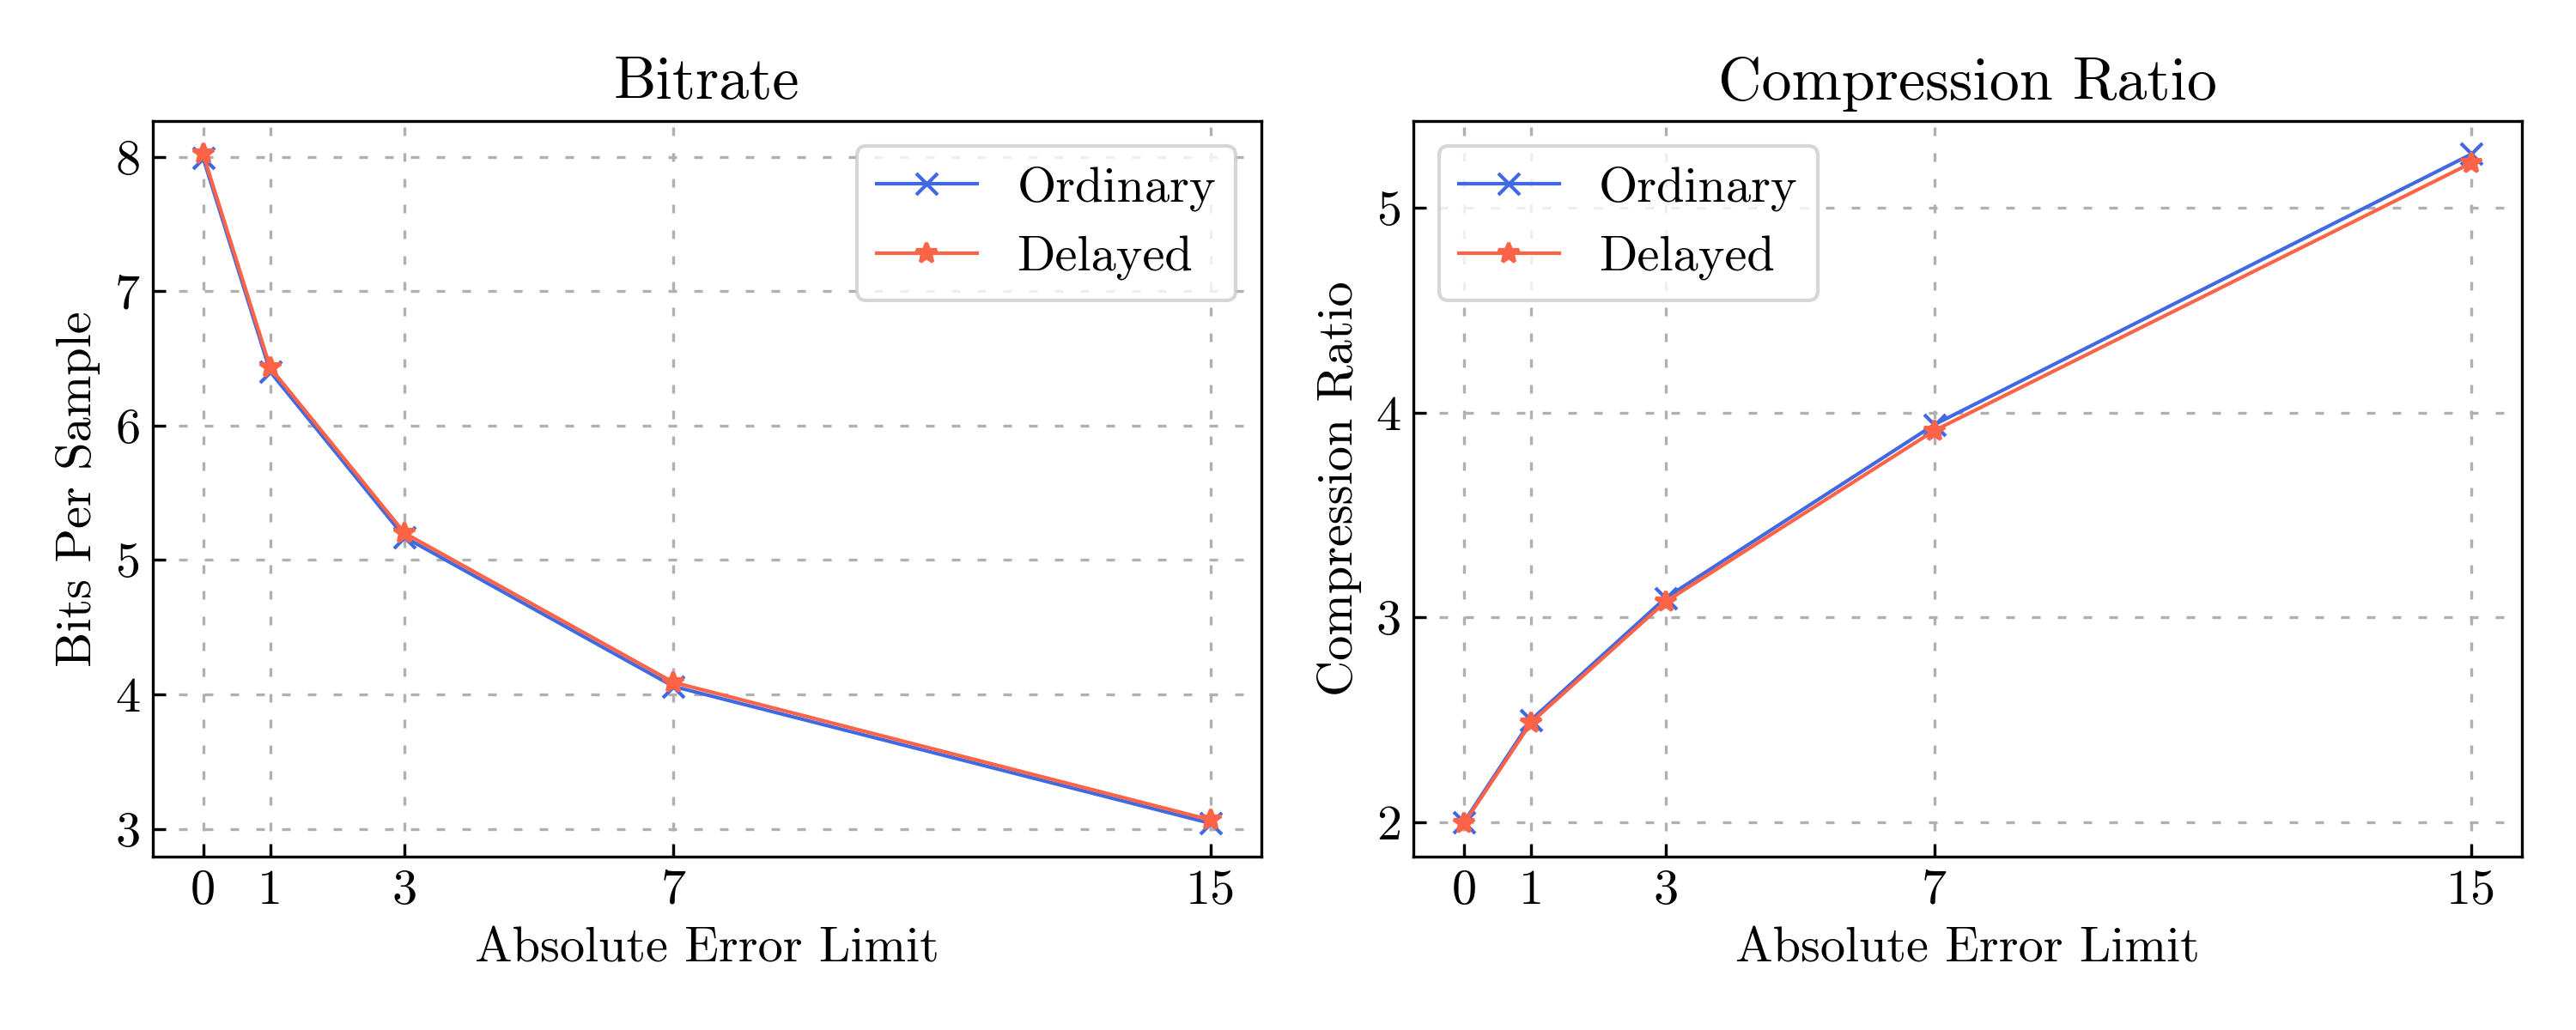
\includegraphics[width=1\textwidth]{figures/compression_performance_hypso.png}
	\end{center}
	\caption{Compression performance presented in bits per sample and compression ratio for a set of absolute error limits. Results are averaged over a set of ten \acrshort{hypso}-2 coastline images with $D=16$.}
	\label{fig:compression-performance-hypso}
\end{figure}

\begin{figure}[ht]
	\begin{center}
		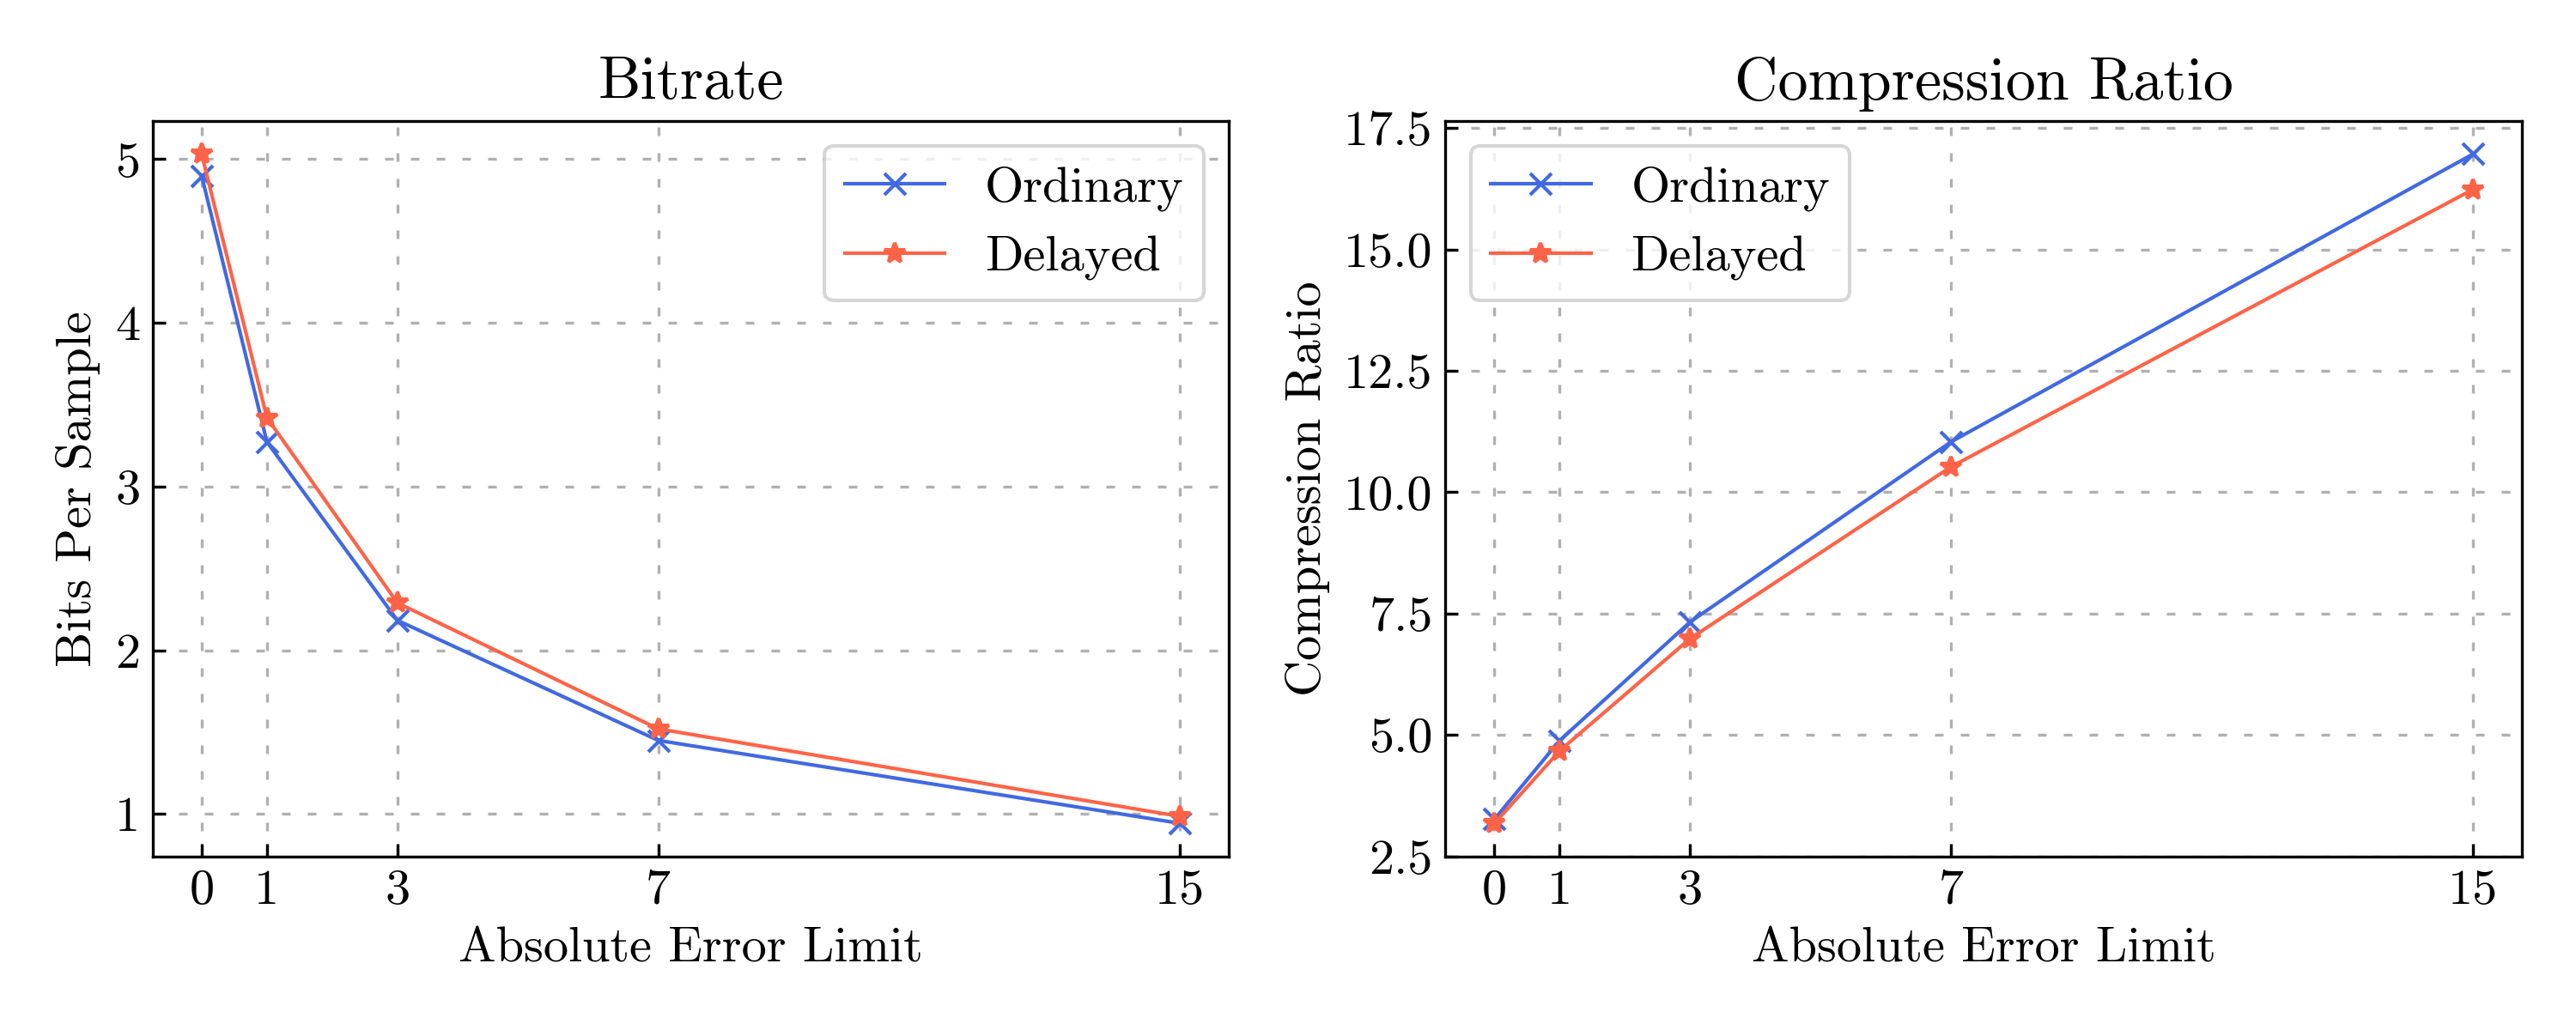
\includegraphics[width=1\textwidth]{figures/compression_performance_aviris.png}
	\end{center}
	\caption{Compression performance presented in bits per sample and compression ratio for a set of absolute error limits. Results are averaged over AVIRIS Yellowstone image set with $D=16$.}
	\label{fig:compression-performance-aviris}
\end{figure}

\begin{table}[ht]
	\caption{PSNR of decompressed images averaged over ten coastline images from HYPSO-2 for a set of PAEs.}
	\label{tab:psnr-compared}
	\begin{center}
		\begin{tabular}{lrr}
			\hline
			\textbf{PAE} & \textbf{CR} & \textbf{PSNR (dB)} \\
			\hline
			0            & 1.995       & N/A                \\ % 2.03            -> 2.02
			1            & 2.488       & 225.86             \\ % 2.55 (225.86dB) -> 2.53 (225.86dB)
			3            & 3.077       & 207.95             \\ % 3.17 (207.95dB) -> 3.15 (207.94dB)
			7            & 3.912       & 192.55             \\ % 4.07 (192.54dB) -> 4.03 (192.54dB)
			15           & 5.219       & 178.08             \\ % 5.45 (178.10dB) -> 5.39 (178.10dB)
			\hline
		\end{tabular}
	\end{center}
\end{table}

\autoref{tab:psnr-compared} shows the \acrshort{PSNR} of reconstructed \acrshort{hypso}-2 images compressed using delayed weight updates. For the lossless mode, reconstructed images are identical. As \acrshort{PAE} increases, the \acrshort{PSNR} drops. Quality of the reconstructed images is not affected by the weight update scheme, and thus the \acrshort{PSNR} for images compressed with the standard compliant weight updates are identical to those of the table.

As opposed to \citeauthor{jiaRemovalFeedbackLoop2025}, this work keeps weights constant across the first samples of each line, rather than each band (\autoref{eq:delayed-weight-updates-modified}). The penalty on compression performance of this modification is evaluated using the verification model. Results are summarized in \autoref{tab:band-line}, and show an insignificant reduction in performance for \acrshort{hypso}-2 coastline images.

\begin{table}[ht]
	\caption{Keeping weights at the start of every line compared with keeping weights only at the start of every band.}
	\label{tab:band-line}
	\begin{center}
		\begin{tabular}{lrr}
			\hline
			\textbf{PAE} & \textbf{Line} & \textbf{Band} \\
			\hline
			0            & 1.995         & 1.995         \\
			1            & 2.488         & 2.488         \\
			3            & 3.077         & 3.078         \\
			7            & 3.912         & 3.913         \\
			15           & 5.219         & 5.219         \\
			\hline
		\end{tabular}
	\end{center}
\end{table}

\begin{figure}[ht!]
	\begin{center}
		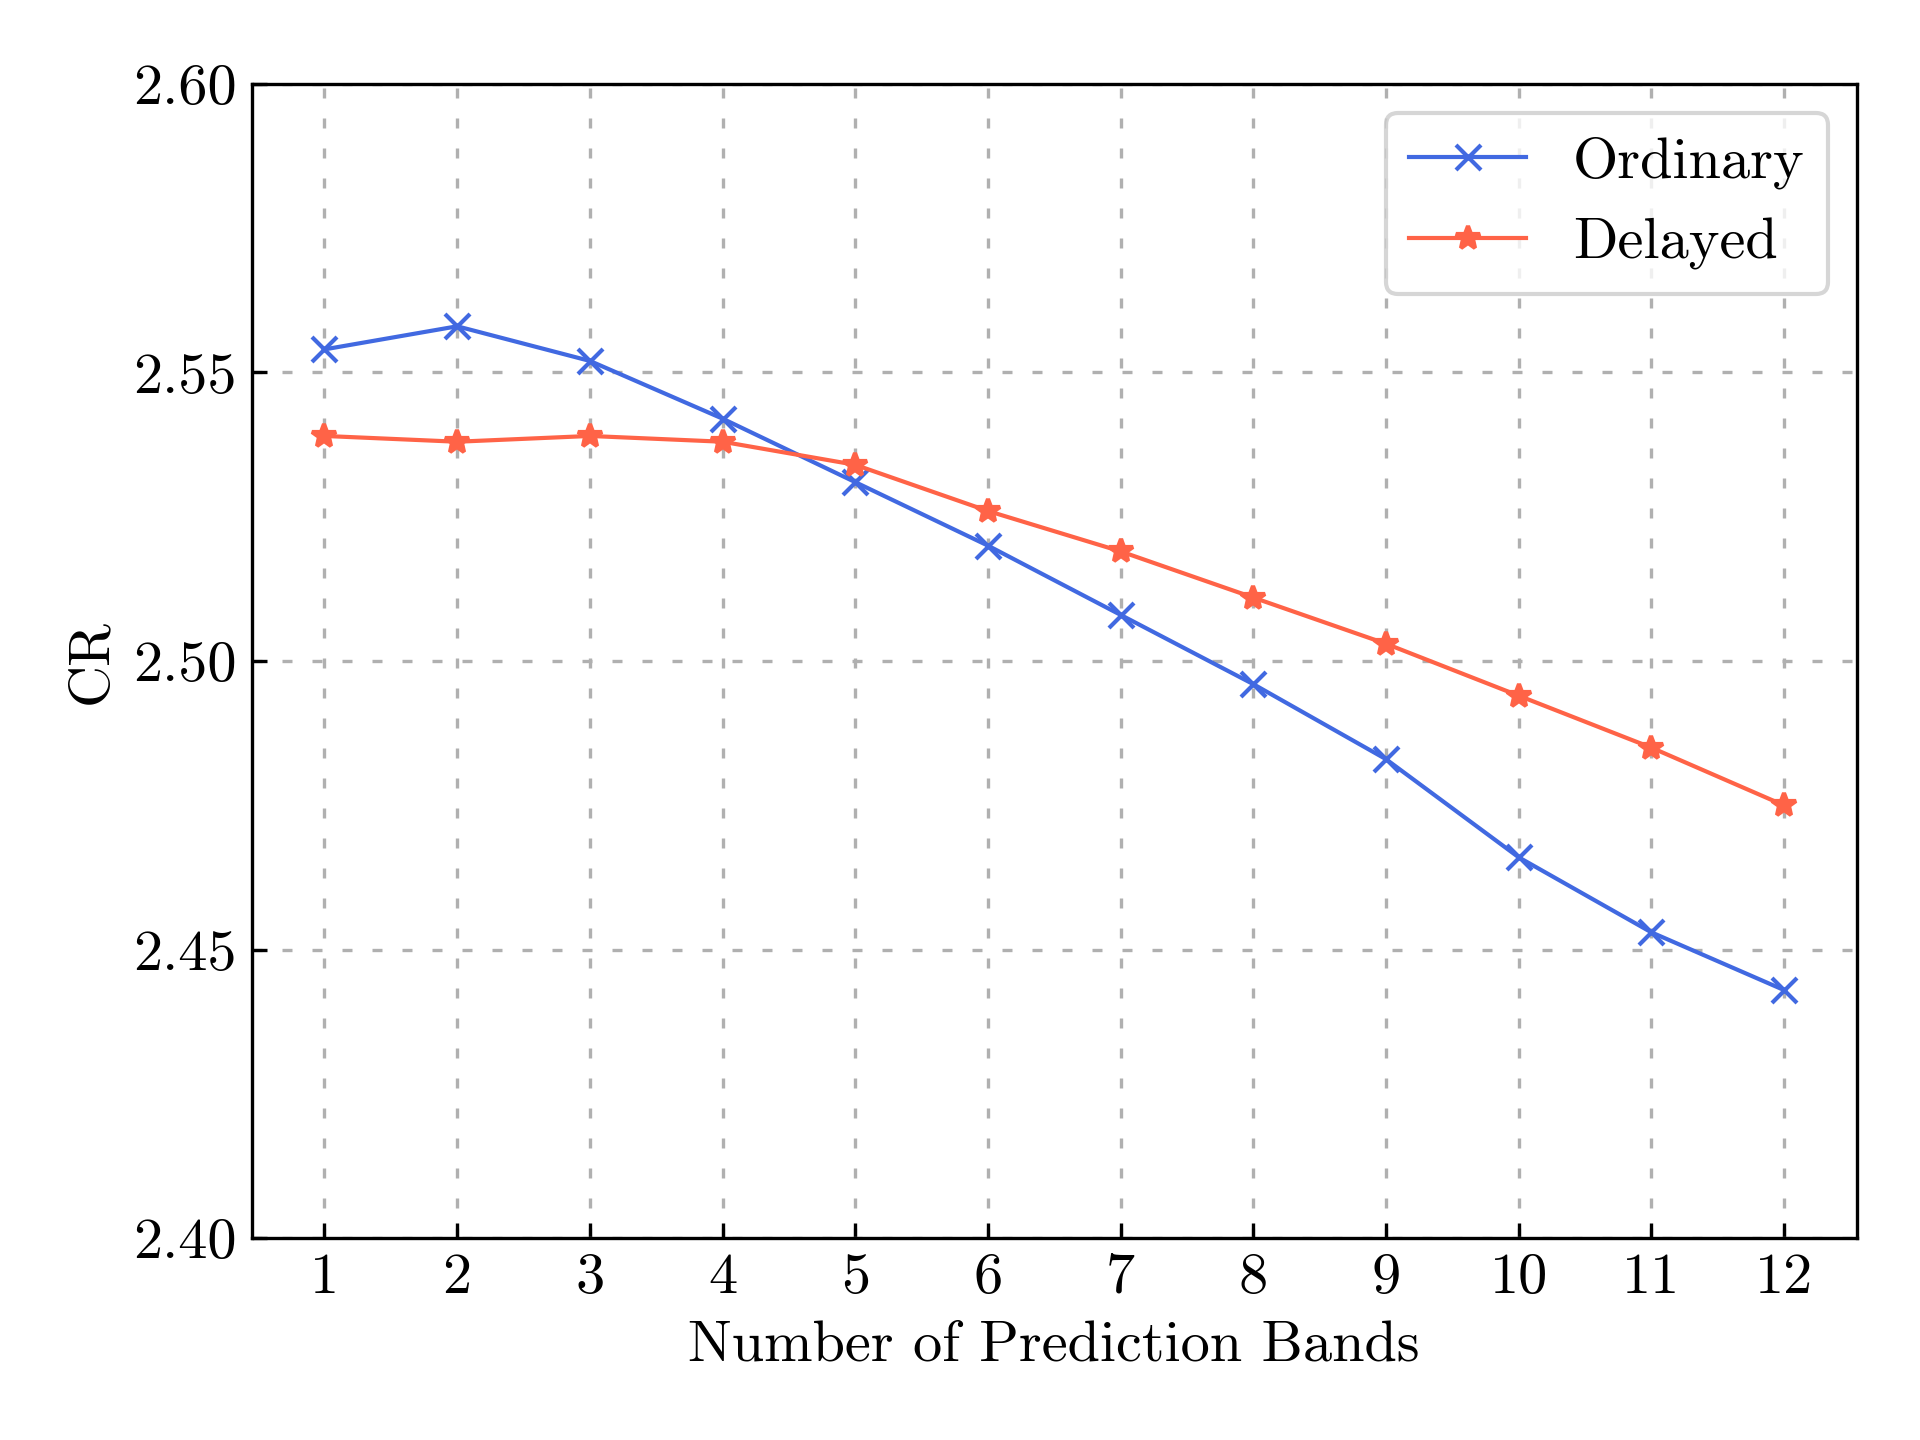
\includegraphics[width=0.6\textwidth]{figures/prediction_bands.png}
	\end{center}
	\caption{Compression performance with $r_z=16$ and $a_z=4$ for different numbers of prediction bands $P$, with and without delayed weight updates. Results are averaged over a set of ten HYPSO-2 coastline images.}
	\label{fig:prediction_bands}
\end{figure}

\autoref{fig:prediction_bands} shows compression ratios with and without delayed weight updates for a range of different numbers of prediction bands. Tests are run for the \acrshort{hypso}-2 image set, with $a_z=4$ and $r_z=16$. For ordinary weight updates, $P=2$ gives the highest compression ratio, with performance dropping as $P$ increases. Delayed weight updates result in a flatter curve, indicating a lower sensitivity to the number of prediction bands, with $P=3$ providing the best results. Interestingly, delayed weight updates outperforms the ordinary scheme for higher numbers of prediction bands.

\section{RTL Results}

The modified hardware accelerator is evaluated using the configuration shown in \autoref{tab:parameters} for two different \acrshort{FPGA}s: Zynq-7030 and Zynq ZU7EV. Results are summarized in \autoref{tab:performance-results-hw} for the whole compression core and the predictor module only. The design is evaluated on hardware resource utilization and estimates of the maximum clock frequency based on static timing analysis. For the Zynq-7030 a maximum clock frequency of 92.6 MHz is reached, and 202 MHz for the Zynq ZU7EV, with the latter reaching realtime processing speed. The predictor module only achieves a significantly higher clock frequency, reaching 351 MHz for the Zynq ZU7EV.

Estimates of the power consumption increase with clock frequency, with 284 mW at the lowest, and 1282 mW at the highest. Different \acrshort{FPGA}s also give different power consumptions at the same frequency, something that is not analysed in this work. The compressor maintains a small area footprint, although slightly larger than that of \citeauthor{vorhaugHyperspectralImageCompression2024}, with 6349 \acrshort{LUT}s and 3480 \acrshort{FF}s for the Zynq ZU7EV.

\begin{table}[ht]
	\caption{Resource utilization, power, and maximum clock frequency of the issue 2 hardware accelerator for two different FPGAs, both for the whole accelerator and only the predictor module.}
	\label{tab:performance-results-hw}
	\begin{center}
		\begin{tabular}{lrrrrrr}
			\hline
			\textbf{FPGA}          & \textbf{LUT} & \textbf{FF} & \textbf{DSP} & \textbf{BRAM} & \textbf{Power} & \textbf{Frequency} \\
			\hline
			Zynq-7030              & 5969         & 3463        & 4            & 83.5          & 284 mW         & 92.6 MHz           \\
			Zynq ZU7EV             & 6349         & 3480        & 4            & 79.5          & 890 mW         & 202.0 MHz          \\
			Zynq-7030 (predictor)  & 2866         & 2250        & 4            & 69.5          & 419 mW         & 137.0 MHz          \\
			Zynq ZU7EV (predictor) & 2807         & 2244        & 4            & 69.5          & 1282 mW        & 350.9 MHz          \\
			\hline
		\end{tabular}
	\end{center}
\end{table}

Static timing analysis shows that the critical path of the updated design lies between the predictor and hybrid encoder modules. The starting point is the shift register buffer for the control signal record in the predictor, which follows the processed sample through the pipeline. The critical path terminates in one of the codeword tables for low-entropy codes in the hybrid encoder. Since the critical path is related to the encoder module, higher clock frequency is achieved for the predictor module in isolation. After splitting the sample representative calculation of stage D+9 (\autoref{fig:new-stageD9}), the critical path of the predictor is once again in the weight update calculation. The path starts and ends at the register storing weights $\omega_z^{(i)}(t)$ for weight updates within lines, shown on the right side of \autoref{fig:weights-hw}. Outputs from the register are processed through the refinement step and clipping before looping back to the register input (\autoref{fig:weights-pipeline-hw}).

\section{On-Board Results}

\begin{figure}[b!]
	\begin{center}
		\efbox{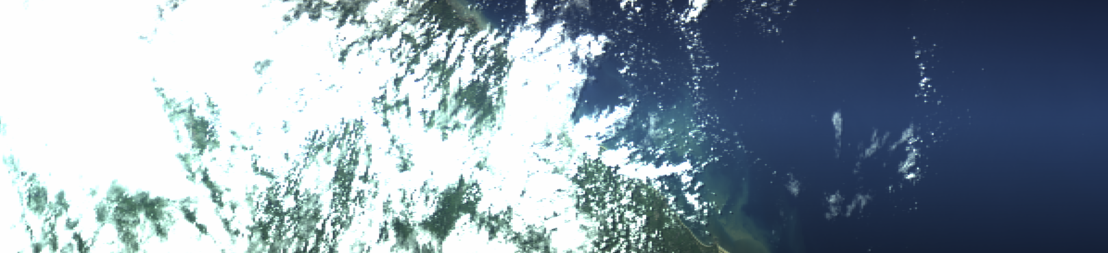
\includegraphics[width=0.8\textwidth]{figures/hypso2-rgb/marceio_onboard_test.png}}
	\end{center}
	\caption{Image captured by the \acrshort{hypso}-2 satellite and compressed on-board using the modified hardware accelerator. The compressed bitstream was decompressed on-ground using the verification model.}
	\label{fig:onboard-test}
\end{figure}

The modified hardware accelerator was tested on-ground using the \acrshort{hypso}-2 engineering model with the configuration presented in \autoref{tab:parameters}. All images from the \acrshort{hypso}-2 coastline set were compressed by hardware, giving identical results as the verification model. After on-ground testing, the design was uplinked to the \acrshort{hypso}-2 satellite. An image of dimensions $N_z=120$, $N_y=598$ and $N_x=1092$ was captured at $8$ frames per second. The image was compressed on-board using the hardware accelerator running at a clock frequency of 92 MHz, downlinked and decompressed on-ground using the verification model. Additionally, the same image was compressed using on-board issue 1 compliant software and downlinked. Using issue 1, the image was compressed with a compression ratio of $2.03$, whereas issue 2 with delayed weight updates achieved a ratio of $2.50$.

The decompressed image, using issue 2, is shown in \autoref{fig:onboard-test}. White areas in the image are clouds which have a high reflection of incoming light, resulting in oversaturated image pixels. The visible coastline in the image is located in Marceió, Brazil. Visual inspection of the decompressed image from issue 1 and 2 show that the accelerator worked on-board the satellite.


% unused tables


% \begin{table}[ht]
% 	\caption{\acrshort{CPU} time and memory use profile for image compression using C++ predictor and reduced memory usage.}
% 	\label{tab:profile-new}
% 	\begin{center}
% 		\begin{tabular}{lrr}
% 			\hline
% 			\textbf{Module} & \textbf{CPU Time} & \textbf{Memory Use} \\
% 			\hline
% 			Total           & 9.4s              & 438MB               \\
% 			Loading         & 0.9\%             & 17.2\%              \\
% 			Predictor       & 72.6\%            & 13.8\%              \\
% 			Hybrid encoder  & 26.4\%            & 69.0\%              \\
% 			Save outputs    & <0.1\%            & N/A                 \\
% 			\hline
% 		\end{tabular}
% 	\end{center}
% \end{table}

% \begin{table}[ht]
% 	\caption{Performance of compression using verification model with C++ predictor and delayed weight updates for single image tests from HYPSO-2, AVIRIS and Landsat with $r_z=16$ and $a_z=4$.}
% 	\label{tab:performance-results-hlm-compress-cpp}
% 	\begin{center}
% 		\begin{tabular}{lrrrrr}
% 			\hline
% 			\textbf{Image} & \textbf{Predictor} & \textbf{Samples} & \textbf{Time (s)} & \textbf{Throughput (MS/s)} & \textbf{Memory (MB)} \\
% 			\hline
% 			HYPSO-2        & C++                & 78361920         & 821               & 0.095                      & 32415                \\ % & (293)
% 			AVIRIS         & C++                & 77643776         & 1166              & 0.066                      & 32091                \\ % & (290)
% 			Landsat        & C++                & 6291456          & 103               & 0.061                      & 2669                 \\ % & (22)
% 			\hline
% 		\end{tabular}
% 	\end{center}
% \end{table}

% \begin{table}[ht]
% 	\caption{Performance of decompression using verification model with C++ predictor and delayed weight updates for single image tests from HYPSO-2, AVIRIS and Landsat with $r_z=16$ and $a_z=4$.}
% 	\label{tab:performance-results-hlm-decompress}
% 	\begin{center}
% 		\begin{tabular}{lrrrr}
% 			\hline
% 			\textbf{Image} & \textbf{Samples} & \textbf{Time (s)} & \textbf{Throughput (MS/s)} & \textbf{Memory (MB)} \\
% 			\hline
% 			Hypso 2        & 78361920         & 1093              & 0.072                      & 32414                \\
% 			AVIRIS         & 77643776         & 1834              & 0.042                      & 32091                \\
% 			Landsat        & 6291456          & 149               & 0.042                      & 2667                 \\
% 			\hline
% 		\end{tabular}
% 	\end{center}
% \end{table}

% \begin{table}[ht]
% 	\caption{Performance of compression using verification model with Python predictor and delayed weight updates for single image tests from HYPSO-2 and Landsat with $r_z=16$ and $a_z=4$.}
% 	\label{tab:performance-results-hlm-compress-py}
% 	\begin{center}
% 		\begin{tabular}{lrrrrr}
% 			\hline
% 			\textbf{Image} & \textbf{Predictor} & \textbf{Samples} & \textbf{Time (s)} & \textbf{Throughput (MS/s)} & \textbf{Memory (MB)} \\
% 			\hline
% 			HYPSO-2        & Python             & 78361920         & 2818              & 0.027                      & 38996                \\ % & (2169)
% 			Landsat        & Python             & 6291456          & 263               & 0.024                      & 3204                 \\ % & (161)
% 			\hline
% 		\end{tabular}
% 	\end{center}
% \end{table}

% \begin{table}[ht]
% 	\caption{Reductions in compression performance for coastline image for this work and the work by \citeauthor{jiaRemovalFeedbackLoop2025}.}
% 	\label{tab:cr-compared}
% 	\begin{center}
% 		\begin{tabular}{lrr}
% 			\hline
% 			PAE & Coastline, \citeauthor{jiaRemovalFeedbackLoop2025} & Coastline, this work \\
% 			\hline
% 			0   & $-1.53\%$                                          & $-0.371\%$           \\ % 2.03            -> 2.02
% 			1   & $-2.88\%$                                          & $-0.470\%$           \\ % 2.55 (225.86dB) -> 2.53 (225.86dB)
% 			3   & $-3.86\%$                                          & $-0.565\%$           \\ % 3.17 (207.95dB) -> 3.15 (207.94dB)
% 			7   & $-4.30\%$                                          & $-0.739\%$           \\ % 4.07 (192.54dB) -> 4.03 (192.54dB)
% 			15  & $-1.23\%$                                          & $-0.826\%$           \\ % 5.45 (178.10dB) -> 5.39 (178.10dB)
% 			\hline
% 		\end{tabular}
% 	\end{center}
% \end{table}

% \begin{figure}[ht]
% 	\begin{center}
% 		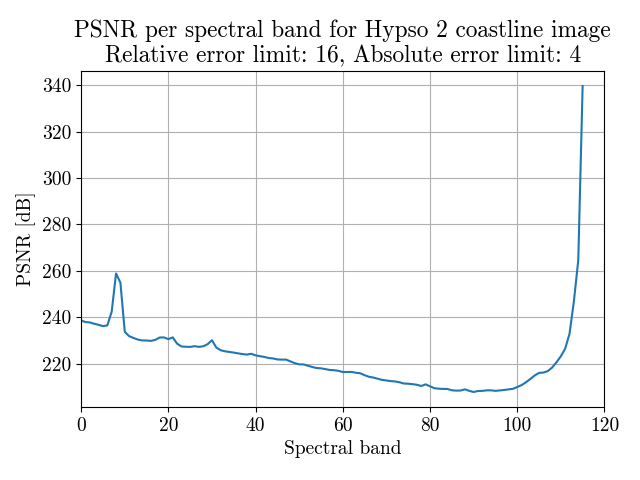
\includegraphics[width=0.65\textwidth]{figures/relative-psnr-coastline.png}
% 	\end{center}
% 	\caption{}
% 	\label{fig:relative-psnr-coastline}
% \end{figure}

% \begin{table}[ht]
% 	\caption{Reduction in compression performance for single image tests with $r_z=16$ and $a_z=4$.}
% 	\label{tab:performance-results-hlm-dw}
% 	\begin{center}
% 		\begin{tabular}{lrrrr}
% 			\hline
% 			\textbf{Image} & \textbf{Ordinary} & \textbf{Delayed} & \textbf{Decrease} \\
% 			\hline
% 			HYPSO-2        & 2.49              & 2.47             & $-0.80\%$         \\
% 			AVIRIS         & 4.41              & 4.31             & $-2.23\%$         \\
% 			Landsat        & 5.21              & 4.82             & $-7.49\%$         \\
% 			\hline
% 		\end{tabular}
% 	\end{center}
% \end{table}
